\documentclass[a4paper, 12pt]{article}
\usepackage{comment} % enables the use of multi-line comments (\ifx \fi) 
\usepackage{fullpage} % changes the margin
\usepackage{sectsty}
\usepackage{graphicx}
\usepackage{dblfloatfix}
\usepackage{float}
\usepackage{listings}
\usepackage{subcaption}
\usepackage{verbatim}
\usepackage{amssymb}
\usepackage{amsmath}
\usepackage{hyperref}
\hypersetup{
    colorlinks=true,
    linkcolor=blue,
    filecolor=magenta,      
    urlcolor=cyan,
}
 
\urlstyle{same}


\sectionfont{\fontsize{13}{15}\selectfont}
\begin{document}
\noindent
\large\textbf{HW 1} \hfill \textbf{Roy Zhang} \\
\normalsize APC 523 \hfill NetID: ruoyaoz \\
Due Date: 03/13/2019 \hfill PUID: 920199846\\

\section{Error in (symmetric) rounding vs. chopping}
The same notation is used to map a real number x to a nearby machine number in $\mathbb{R}(p,q)$ as discussed in class. If we expand the binary scientific notation, we have
\[x = m \times 2^e = \pm (\sum ^\infty _{l=1} b_{-l}2^{-l})\times 2^e \]
, where $m$ is $p$ bits of mentissa and $e$ is $q$ bits of exponent. The claim from the question is that

\[\vert \frac{x-rd(x)}{x} \vert \leq 2^{-p} \]

Now we should consider the following two cases where the first discarded bit is either 0 or 1.

\subsection{$b_{p+1}=0$}

If the first discarded bit ($p+1$ term) is 0, then

\[rd(x) = \pm (\sum ^{p+1} _{l=1} b_{-l}2^{-l})\times 2^e\]
\[x-rd(x) = \pm (\sum ^\infty _{l=p+2} b_{-l}2^{-l})\times 2^e\]

Taking the maximum value of the absolute value of $x-rd(x)$, we have

\[\vert x-rd(x) \vert _{max}=\sum ^\infty _{l=p+2} 2^{-l})\times 2^e = 2^{-p-1}\times 2^e = 2^{e-p-1}\]

, where all the bits from $p+2$ to $\infty$ are 1s. Then we assume the value of mentissa is the smallest possible number can be represented using this notation if it is not zero. $m_{min} = (.10000...)_2$. Therefore,

\[\vert \frac{x-rd(x)}{x} \vert _{max} = \frac{2^{e-p-1}}{2^{-1}\times 2^e} = 2^{-p}\]

Since any non-zero mentissa has a value larger or equal than this, so the relative error of this case is

\[\vert \frac{x-rd(x)}{x} \vert _{max} \leq 2^{-p}\]



\subsection{$b_{p+1}=1$}

If the first discarded bit is 1, we round up. So $rd(x)$ is 

\[rd(x) = (\sum ^{p+1}_{l=1} b_{-l}e^{-l} + 2^{-(p+1)})*2^e\]

The rounding up is performed by adding 1 to the $(p+1)$th term, which will be a 0 after addition. So,

\[x-rd(x) = \pm (\sum ^\infty _{l=p+2} b_{-l}2^{-l} - 2^{-p-1})\times 2^e\]

Maximize the difference, we have

\[\vert x-rd(x) \vert _{max} = 2^{-p-1}\times 2^e = 2^{e-p-1}\]

Then, just as the previous section, 

\[\vert \frac{x-rd(x)}{x} \vert _{max} = \frac{2^{e-p-1}}{2^{-1}\times 2^e} = 2^{-p}\]

\[\vert \frac{x-rd(x)}{x} \vert _{max} \leq 2^{-p}\]

Therefore, it is proven that the upper bound in the relative error for symmetric rounding is as stated in the claim.

\section{An accurate implementation of $e^x$}


\subsection*{(a)}
Using the Matlab code as listed in Appendix 2a (q2.m), the sum of the first 31 terms with 5 significant figures is

\[e^{5.5} = 244.71\]

\subsection*{(b)}
By working out the partial sums, we find that for $k = 18$ and beyond, the value of $e^{5.5}$ converges to five significant figures, which equals $244.71$. This means adding the 18th term does not change the sum. With the built-in function at double precision, we have
\[e^{5.5} = 2.446919322642204\times 10^2\]

and the relative error is
\[RE =\frac{|244.71-e^{5.5}|}{e^{5.5}} \approx 7.383870654188337\times 10^{-5}\]

\subsection*{(c)}

When adding the terms from right to left, it is found that the result now converges at $k = 22$ with the same value

\[e^{5.5} = 244.71\]

Thus, the same relative error.

\subsection*{(d)}
The MATLAB code is q2.m


\subsubsection*{(i)}

For $k=26$ and beyond, the results added from left to right converge to value
\[e^{-5.5} \approx 0.0038363\]

\subsubsection*{(ii)}
For $k=20$ and beyond, the results added from right to left converge to value

\[e^{-5.5} \approx 0.0040000\]


\subsubsection*{(iii)}
When adding both positive terms and negative terms seperately from left to right and then combining the two, the result converges at $k = 18$ and beyond with value

\[e^{-5.5} \approx 0.0\]


\subsubsection*{(iv)}

When adding both positive terms and negative terms seperately from right to left and then combining the two, the result converges at $k = 19$ and beyond with value

\[e^{-5.5} \approx 0.010000\]

From (i) to (iv), we can see that, for positive summation, adding from right to left converges faster; for negative summation, adding from left to right converges faster. As shown by part (b), when exponent is positive and adding from left to right has the lowest error.\\

Instead of computing $e^{-x}$, we can compute $\frac{1}{e^{x}}$ to avoid negative exponent or negative summation. The result is $\frac{1}{e^{x}} \approx 0.0040865$, which is more accurate than any of the method used in part (d).


\section{Error propagation in exponentiation}


\subsection*{(a) Whole-number exponent}
Let $fl(x)$ be the floating point representation of $x\in \mathbb{R}(p,q)$. Operations on 2 machine numbers produce a machine number
\[fl(x\circ y) = (x\circ y)(1+\epsilon)\]

, where $|\epsilon| \leq eps$.

\subsubsection*{(i) Repeatedly multiplying by x}

\[fl(x\times x) = x^2(1+\epsilon)\]
\[fl(x^3)=fl[x\times fl(x\times x)] = fl[x\times x^2(1+\epsilon)] = x^3 (1+\epsilon)(1+\epsilon) = x^3(1+2\epsilon+ \epsilon ^2)\]

If we neglect terms of $O(eps^2)$,

\[fl(x^3) \approx x^3(1+2\epsilon)\]
\[fl(x^4) = x\times fl(x^3) = x^4(1+2\epsilon)(1+\epsilon)= x^4 (1+3\epsilon +O(\epsilon^2))\approx x^4 (1+3\epsilon)\]

Repeat the multiplication for n times,
\[fl(x^n) = fl[x\times fl(x^{n-1})] = x^n[1+(n-1)\epsilon]\]

\subsubsection*{(ii) Computing $e^{nln(x)}$}

\[fl(lnx)=ln(x)(1+\epsilon)\]

Neglect terms of $O(eps^2)$ as above,
\[fl(nln(x)) = fl[n\times fl(lnx)] = fl[n\times ln(x)(1+\epsilon)]=nln(x)(1+\epsilon)^2\approx nln(x)(1+2\epsilon)\]

\[fl[e^{fl(nlnx)}]= fl[e^{nln(x)(1+2\epsilon)}] = fl[e^{nln(x)}\times e^{2\epsilon}] = x^ne^{2\epsilon}(1+\epsilon)\]

Expand the term $e^{2\epsilon}$ and ignore $O(eps^2)$,

\[e^{2\epsilon}\approx 1 + 2\epsilon\]

Then,

\[fl[e^{fl(nlnx)}]\approx x^n(1+2\epsilon)(1+\epsilon) \approx x^n(1+3\epsilon)\]


When comparing the results for two methods for exponentiation, we can see that when $n<4$, i.e. $n-1<3$, calculation via repeated multiplication is more accurate than the log-exponential method; when $n=4$, two methods yield comparable error; for $n>4$, the log-exponential method will be more accurate.

\subsection*{(b) Arbitrary components}

\subsubsection*{(i)}
Let's assume $x$ is an exact number and $a = a(1+\epsilon _a)$, so

\[x^a = x^{a(1+\epsilon _a)} = x^a x^{a\epsilon_a} = x^a e^{a\epsilon_a ln(x)}\]

Then, expand $e^{a\epsilon_a ln(x)}$ as

\[e^{a\epsilon_a ln(x)} = 1+ a\epsilon_a ln(x) +O(\epsilon_a ^2)\]

So,

\[x^{a(1+\epsilon _a)} \approx x^a[1+a\epsilon_a ln(x)]\]

\subsubsection*{(ii)}

Assume $a$ is an exact machine number and $x = x(1+\epsilon_x)$.

\[x^a = [x(1+\epsilon _x)]^a = x^a (1+\epsilon_x)^a\]

If neglecting terms that are above first-order in $\epsilon _x$,

\[x^a = [x(1+\epsilon _x)]^a \approx x^a (1+a\epsilon_x)\]

For (i), if $|a|$ is large and/or x approaches either $0$ or $\infty$ ($lnx$ diverges), the propagated error can be substantial. For (ii), if $|a|$ is large, the propagated error can be substantial.

\section{Conditioning}

\subsection*{(a)}
From definition,
\[(cond\ f)(x) = | \frac{xf'(x)}{f(x)} |\]
For
\[f(x)=1-e^{-x}\]
\[f'(x) = e^{-x}\]
Therefore, in the interval $[0,1]$,
\[(cond\ f)(x) = | \frac{xf'(x)}{f(x)} | = |\frac{xe^{-x}}{1-e^{-x}}| = |\frac{x}{e^x-1}| = \frac{x}{e^x-1}\]

If expanding $e^x$, we have $e^x = 1 + x + \frac{x^2}{2!} + \frac{x^3}{3!} + ...$, thus $e^x-1 > x$. Therefore, it is proven that

\[(cond\ f)(x) =\frac{x}{e^x-1} < 1\]

\subsection*{(b)}
Set $\epsilon _e$ for exponentiation and $\epsilon_s$ for subtraction.

\[f_A(x) = [1-e^{-x}(1+\epsilon_e)](1+\epsilon_s)=1+\epsilon_s - e^{-x}(1+\epsilon_e+\epsilon_s+\epsilon_s\epsilon_e)\]

, where $\epsilon_s\epsilon_e$ can be neglected,
\[f_A(x) = 1-e^{-x}+\epsilon_s -(\epsilon_e+\epsilon_s)e^{-x}\]

Now we set $f_A(x)=f(x_A)$, where $f(x_A)=1-e^{-x_A}$. Hence,

\[1-e^{-x}+\epsilon_s -(\epsilon_e+\epsilon_s)e^{-x} = 1-e^{-x_A}\]

\[e^{-x_A} = e^{-x}-\epsilon_s + (\epsilon _e +\epsilon _s)e^{-x}\]
\[-x_A = -x + ln(1+\epsilon_e +\epsilon_s-\frac{\epsilon _s}{e^{-x}})\]
\[x-x_A = ln(1+\epsilon_e +\epsilon_s-\epsilon_s e^{x})\]

We then expand the natural log term and ignore the high order $\epsilon$ terms as following,
\[ln(1+\epsilon_e +\epsilon_s-\epsilon_s e^{x}) \approx \epsilon_e +\epsilon_s-\epsilon_s e^{x}\]

Plug in to the equation above and divide both sides by $x$,

\[\frac{x-x_A}{x}= \frac{\epsilon_e +\epsilon_s-\epsilon_s e^{x}}{x}\]

As definition, $(cond\ A)(x) = \frac{1}{eps} |\frac{x-x_A}{x}|$. To find the upper bound of $(cond\ A)(x)$, we want to maximize the RHS. Since $|\epsilon_s|=|\epsilon_e| = eps$, we can choose $\epsilon_e = +\epsilon$ and $\epsilon_s = -\epsilon$, such that $\epsilon_e +\epsilon_s = 0$. Then,

\[(cond\ A)(x) = \frac{|\frac{x-x_A}{x}|}{eps} = \frac{eps - eps -eps\times e^{x}}{x}\times \frac{1}{eps}\]
\[(cond\ A)(x) = \frac{e^x}{x}\]

We know that $\frac{e^x}{x} > 1$ because if we expand $e^x$, we have

\[\frac{1+x+\frac{x^2}{2!}+...}{x} = \frac{1}{x} + 1 + ... \]

Therefore, $(cond\ A)(x)$ is greater than 1 everywhere on $[0,1]$.
\subsection*{(c)}
As shown in the figure below, $(cond\ A)(x)$ and $(cond\ f)(x)$ are plotted. To demonstrate the fact that $(cond\ A)(x)$ is always above 1 and $(cond\ f)(x)$ is always below 1 in the interval, Fig.1b provides a zoomed-in view.


\begin{figure}[H]
    \centering
    \begin{subfigure}[b]{0.45\textwidth}
        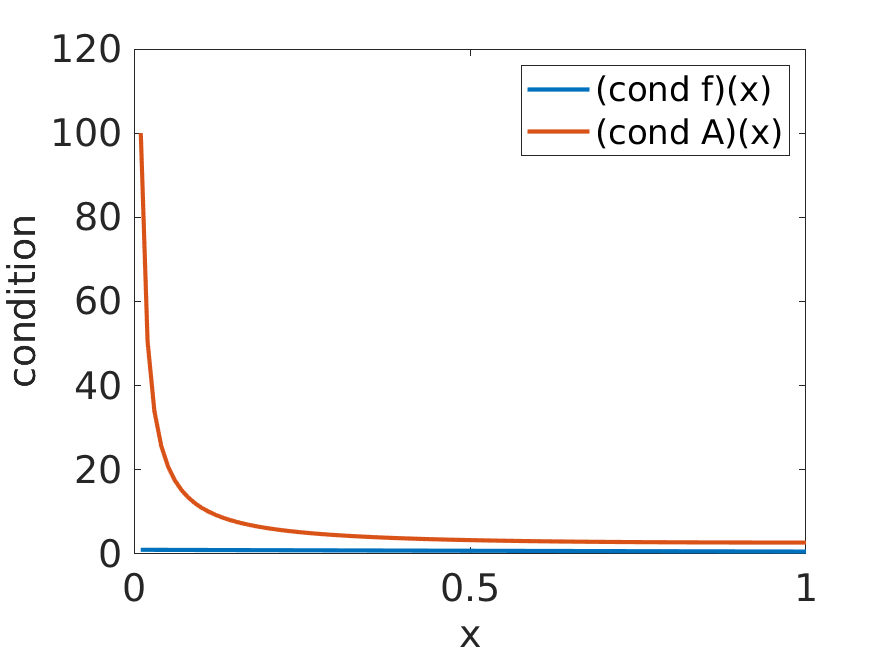
\includegraphics[width=\textwidth]{q4_full.png}
        \caption{Interval $[0,1]$}
        \label{fig:full}
    \end{subfigure}
    ~ 
    \begin{subfigure}[b]{0.45\textwidth}
        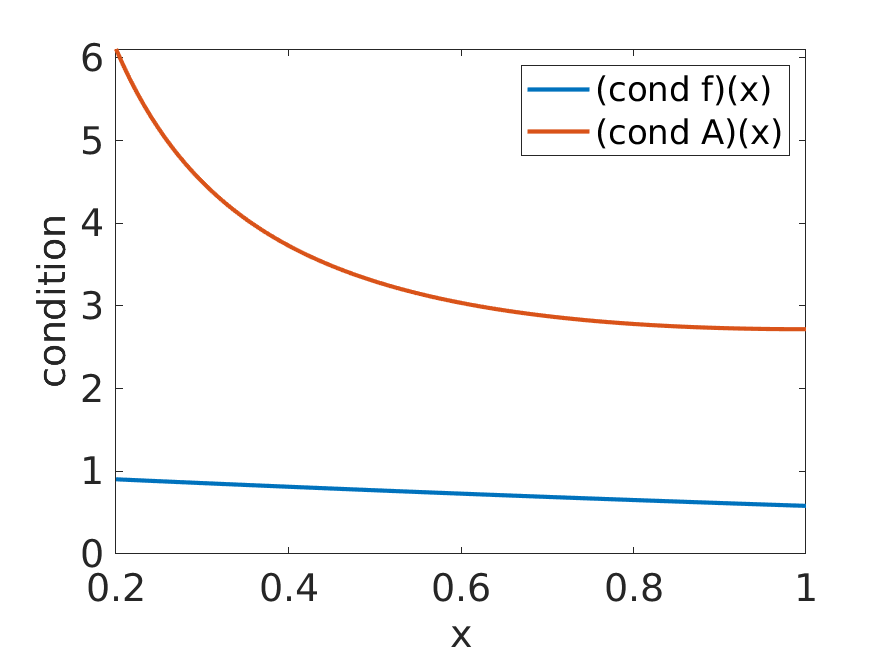
\includegraphics[width=\textwidth]{q4_zoom.png}
        \caption{Interval $[0.2,1]$}
        \label{fig:zoom}
    \end{subfigure}
	\caption{$(cond\ f)(x)$ and $(cond\ A)(x)$ vs. $x$ on $[0,1]$}
	\label{fig:condition}
\end{figure}

We can see that when x is small, A becomes progressively more ill-conditioned. This is because the function $1-e^{-x}$ introduces large error when x is small, which means $e^{-x}$ approaches 1 and the subtraction can cause large error.

\subsection*{(d)}


\subsection*{(e)}


\subsection*{(f)}



\section{Limits in $\mathbb{R}(p,q)$}

The code for this question is listed:

\begin{tiny}
\lstinputlisting[language=Matlab]{q5.m}
\end{tiny}

The output from the is as shown in the table below, where ``pow" means the integral power of 10.

\begin{table}[H]
\centering
\begin{tabular}{|c|c|}
\hline
\textbf{pow} & \textbf{e}     \\ \hline
0            & 2.000000000000 \\ \hline
1            & 2.593742460100 \\ \hline
2            & 2.704813829422 \\ \hline
3            & 2.716923932236 \\ \hline
4            & 2.718145926825 \\ \hline
5            & 2.718268237192 \\ \hline
6            & 2.718280469096 \\ \hline
7            & 2.718281694132 \\ \hline
8            & 2.718281798347 \\ \hline
9            & 2.718282052012 \\ \hline
10           & 2.718282053235 \\ \hline
11           & 2.718282053357 \\ \hline
12           & 2.718523496037 \\ \hline
13           & 2.716110034087 \\ \hline
14           & 2.716110034087 \\ \hline
15           & 3.035035206549 \\ \hline
16           & 1.000000000000 \\ \hline
17           & 1.000000000000 \\ \hline
\end{tabular}
\end{table}



\section{Fun with square roots}

\begin{figure}[H]
	\centering
	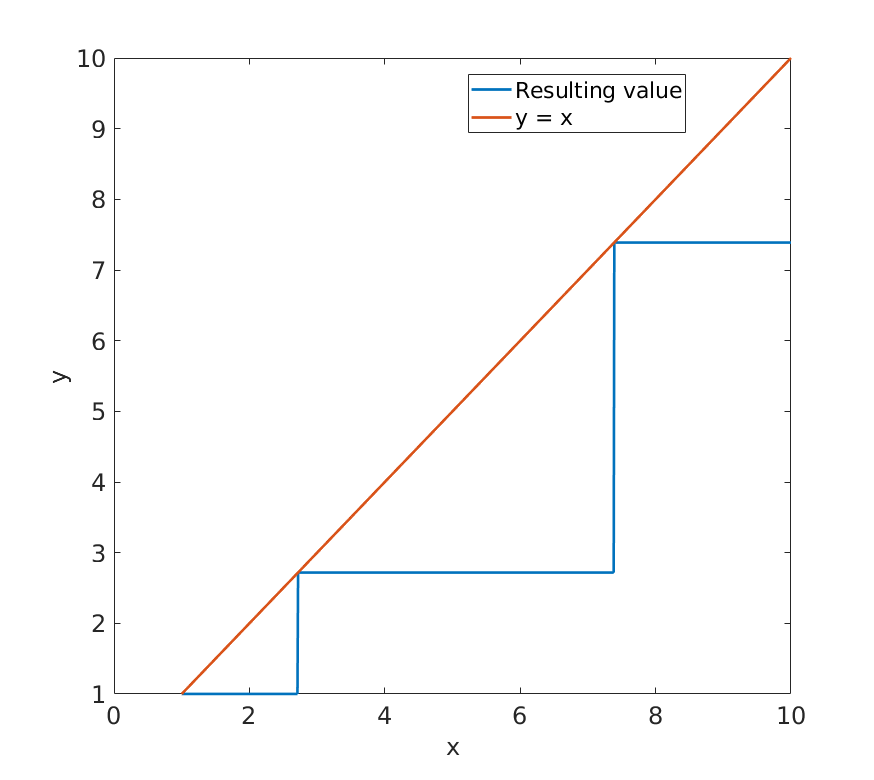
\includegraphics[width=0.7\textwidth]{q6.png}
	\caption{Plot of theoretical value and resulting value of calculation}
	\centering
	\label{fig:2a_pd}
\end{figure}

\section{The issue with polynomial roots}

\subsection*{(a)}

Using the symbolic function in MATLAB and expanding the terms, the coefficients for the polynomial can be obtained as shown below.

\[
\begin{split}
&w(x)=x^{20} - 210*x^{19} + 20615*x^{18} - 1256850*x^{17} + 53327946*x^{16} - 1672280820*x^{15}\\
& + 40171771630*x^{14} - 756111184500*x^{13} + 11310276995381*x^{12} - 135585182899530*x^{11}\\
& + 1307535010540395*x^{10} - 10142299865511450*x^{9} + 63030812099294896*x^{8} \\
& - 311333643161390640*x^{7} + 1206647803780373360*x^{6} - 3599979517947607200*x^{5} \\
& + 8037811822645051776*x^{4} - 12870931245150988800*x^{3} + 13803759753640704000*x^{2} \\
& - 8752948036761600000*x + 2432902008176640000
\end{split}
\]

\subsection*{(b)}
It is found that using different python functions gives different results. The two methods are discussed below.

\subsubsection*{(i) scipy.optimize.newton()}

The python scipy.optimize.newton() function is used to implement Newton-Raphson method with the additional input of the derivative of the polynomial (Man page for the function: \url{https://docs.scipy.org/doc/scipy/reference/generated/scipy.optimize.newton.html}). With an initial guess of 21 and maximum number of iterations set to be 10,000, the root is found after convergence.
\[root = 19.99996633706258\]

We can see that the result is close but not exactly 20 at convergence.

\subsubsection*{(ii) numpy.roots()}

The function numpy.roots() is much more straight-forward. By storing the coefficients in a list, the function returns all the roots (complex).
\[root = 19.999809291236637\]

We can see that method (i) yields a result closer to 20 than method (ii).

\subsection*{(c)}

The result for different $\delta$ is summarized in the table below.

\begin{table}[H]
\centering
\begin{tabular}{|c|c|c|}
\hline
\textbf{$\delta$} & \textbf{Largest root method(i)} & \textbf{Largest root method(ii)} \\ \hline
$10^{-8}$     & 9.584736894572401  & 20.647582887998496+1.1869261883090942j\\ \hline
$10^{-6}$     & 7.752681351742437 & 23.149016041505767+2.740984630381872j\\ \hline
$10^{-4}$     & 5.969335437509083 & 28.40021241591655+6.5104342165628175j\\ \hline
$10^{-2}$     & 5.469592984972789 & 38.478183617151515+20.83432358712749j\\ \hline
\end{tabular}
\end{table}

For method (i), as the value of $\delta$ increases, the largest root found decreases. When comparing with the result from (b), we notice that a perturbation as small as $10^{-8}$ will have huge effect on the largest root, and the effect can be amplified by further increasing $\delta$.\\

For method (ii), which will be used to investigate further questions, shows the opposite behavior. As the value of $\delta$ increases, the largest root found also increases if we only concern about the real part of the root.

\subsection*{(d)}
If we change $a_{19}$ from $-210$ to $-210-2^{-23}$, we have 16th and 17th root as

\[root_{17} = 16.73074487979267+2.812624896721978j\]
\[root_{16} = 16.73074487979267-2.812624896721978j\]

We can see that they are each other's complex conjugate.


\subsection*{(e)}
\subsubsection*{(i)}



\subsubsection*{(ii)}



\subsubsection*{(iii)}


\section{Recurrence in reverse}


\subsection*{(a)}
\[y_{n+1} = e-(n+1)y_n\]
\[y_n = \frac{e-y_{n+1}}{n+1}\]

To reverse the recurrence, let $y_{n+1}$ be $y_n$ for better representation, it becomes
\[y_{n-1} = \frac{e-y_n}{n} = \frac{e}{n}-\frac{y_n}{n}\]
For $y_{n-2}$,
\[y_{n-2} = \frac{e-y_{n-1}}{n-1} = \frac{e-\frac{e-y_n}{n}}{n-1}=\frac{(n-1)e-y_n}{n(n-1)}= \frac{e}{n}-\frac{y_n}{n(n-1)}\]

\[y_{n-3} = \frac{(n-1)^2e-y_n}{n(n-1)(n-2)}=\frac{(n-1)e}{n(n-2)}-\frac{y_n}{n(n-1)(n-2)}\]
If we see this as a map $g_k$ from $y_N$ to $y_k$, from the above trend we can see that
\[y_k = \frac{k!}{N!}y_N + f(N)\]
, where $f(N)$ is some function of $N$. Therefore,
\[(cond\ g_k)(y_N) = |\frac{y_Ny_k'}{g_k}| \leq \frac{k!}{N!}\]


\subsection*{(b)}
\[\epsilon_k = \frac{k!}{N!}\epsilon_N\]
For $\epsilon_N = 100\%$, let relative error in $y_k$ be just $\epsilon$,
\[\epsilon \geq \frac{k!}{N!}\]
\[N! \geq \frac{k!}{\epsilon}\]

\subsection*{(c)}

The machine epsilon for double precision is $2.22\times 10^{-16}$. Using a little piece of code in MATLAB, N is found to be 32.


\subsection*{(d)}
Since $k = 20$, let the loop be from $N = 32$ to $N = 21$. We have
\[y_{MATLAB} = 0.123803830762570\]

Using Wolfram Alpha, we have

\[y_{WA} = 0.123803830762569948691396169958222451199785308141796375457 \approx 0.123803830762570\]

Therefore, two results agree.

%\newpage
%\section*{Appendix}

%\subsection*{Question 2a: q2.m}

%\lstinputlisting[language=Matlab]{q2.m}


%\subsection*{Question 6: q6.m}

%\begin{tiny}
%\lstinputlisting[language=Matlab]{q6.m}
%\end{tiny}


\end{document}
